\documentclass[conference]{IEEEtran}
\IEEEoverridecommandlockouts
% The preceding line is only needed to identify funding in the first footnote. If that is unneeded, please comment it out.
\usepackage{cite}
\usepackage{amsmath,amssymb,amsfonts}
\usepackage{algorithmic}
\usepackage{graphicx}
\usepackage{textcomp}
\usepackage{xcolor}
\def\BibTeX{{\rm B\kern-.05em{\sc i\kern-.025em b}\kern-.08em
    T\kern-.1667em\lower.7ex\hbox{E}\kern-.125emX}}
\begin{document}

\title{Proyecto: Algoritmos Genéticos\\

\thanks{}
}

\author{\IEEEauthorblockN{1\textsuperscript{st} Mauricio Campos Cerdas}

\and
\IEEEauthorblockN{2\textsuperscript{nd} Ian Murillo Campos}

\and
\IEEEauthorblockN{3\textsuperscript{nd} Esteban Villavicencio Soto}

}

\maketitle





\section{Resumen}
Este artículo servirá para relatar el proceso de elaboración de un proyecto realizado en el lenguaje de programación JavaScript, el cual tratará de vectorizar imagenes mediante el uso de un algoritmo genetico, el objetivo final es que el proyecto sea capaz de reproducir un dibujo lineal a partir de una imagen en blanco y negro (1 bit) mediante el retorno de una lista de coordenadas (x, y) que identifiquen los puntos de la linea del dibujo, luego, se expondrán resultados de pruebas de rendimiento para ver como se desempeña en comparación a otros algoritmos que realizan la isma función.


\textbf{Palabras clave:} algoritmo, genético, fitness, población, generación, tiempo, ejecución, imagen.
\section{Introducción}

"Los algoritmos genéticos (AGs) son técnicas de búsqueda y optimización inspiradas en la naturaleza que utilizan propiedades como la herencia, mutación, selección y cruce. Una de las cualidades principales de los algoritmos genéticos es su grado de paralelismo implícito, ya que se trabaja con un conjunto de soluciones de forma simultánea. Al igual que en la naturaleza, la evolución de los individuos no depende únicamente de ellos, sino también de la población a la que pertenecen." [2]

En el proyecto de vectorización de imágenes, este enfoque paralelo de los algoritmos genéticos se vuelve crucial, ya que permite trabajar con múltiples soluciones simultáneamente, buscando la convergencia hacia la representación óptima de la imagen. Esta característica refleja la idea de que la adaptación y mejora no solo dependen de los individuos en sí, sino también de la dinámica de toda la población, estableciendo un paralelismo con el proceso evolutivo en la naturaleza. En otras palabras, los algoritmos genéticos, al incorporar conceptos como la selección natural, herencia y mutación, se convierten en herramientas poderosas para abordar la vectorización de imágenes, permitiendo la evolución simultánea de individuos para obtener la mejor respuesta. 

Para esta sección, se amplió la comprensión de los algoritmos genéticos a través de la revisión detallada proporcionada en el paper titulado "A review on genetic algorithm: past, present, and future" de Sourabh Katoch, Sumit Singh Chauhan y Vijay Kumar[1]. Este estudio nos ha brindado una visión más completa sobre el pasado, presente y futuro de los algoritmos genéticos, inspirando su aplicación en el proyecto actual de vectorización de imágenes. El paper en un detalle interesante presenta que se abordan diversos dominios de investigación relacionados con algoritmos genéticos y se discuten las direcciones futuras en áreas como operadores genéticos, funciones de aptitud y algoritmos híbridos. Este enfoque estructurado se plantea como una herramienta valiosa para la investigación y la enseñanza de posgrado.

En general, el documento ofrece una visión estructurada y detallada de los algoritmos genéticos y sus variantes, discutiendo sus aplicaciones específicas y operadores genéticos diseñados para representación. Se profundiza en el papel de operadores genéticos como crossover, mutación y selección en la mitigación de la convergencia prematura. La aplicabilidad de los algoritmos genéticos en diversos dominios de investigación se discute, resaltando la atención en aplicaciones multimedia y redes inalámbricas. El paper aborda desafíos y problemas que guiarán a los profesionales en sus investigaciones, destacando las ventajas de utilizar algoritmos genéticos en otros dominios de investigación y algoritmos metaheurísticos. En resumen, proporciona no solo la fuente de investigación reciente en algoritmos genéticos, sino también información detallada sobre cada componente de estos algoritmos, alentando a los investigadores a comprender los fundamentos y aplicar ese conocimiento en sus problemas de investigación.



El propósito central de este proyecto es la implementación de un algoritmo genético que, a partir de una imagen en blanco y negro, pueda reproducir un dibujo lineal. Esta tarea implica la generación de una población de individuos que evolucionan a lo largo de sucesivas generaciones. Cada individuo se define como una versión de la lista de coordenadas, ajustándose continuamente hasta converger en laimagen objetivo. Se debe crear una función fitness que debe arrojar un único número que cuantifique la representación de la misma. 
El proyecto se realizará utilizando el lenguaje de programación JavaScript mayoritariamente, apoyándose del lenguaje HTML para crear un entorno gráfico funcional desde la web, la página recibirá desde los archivos del usuario la imagen a replicar y desde ahí se podrán modificar iteraciones del código, entre otros factores hasta llegar a replicar la imagen y retornar la lista de coordenadas. También puede hacer uso de bibliotecas como OpenCV.js y aplicar filtros raster, excluyendo la vectorización de la imagen. 

\section{Propuesta}
Aqui se busca explicar un poco más como se utilizó los algoritmos genéticos en el trabajo. Se muestra primeramente “Individuo” y “Población”, donde la primera funciona como un generador de puntos y la segunda para recolectar y manipular dichos puntos posteriormente. 

La siguiente parte del código contiene funciones para conseguir el valor de los sliders, los cuales son ajustados por el usuario. La finalidad de estos es servir como parámetros del algoritmo genético, aquí encontramos la cantidad de individuos por población, la cantidad de generaciones, el porcentaje de individuos seleccionados, mutados y mezclados.

Una vez carga la imagen, se comprueba que los porcentajes digitados por el usuario sean iguales a 100. Si lo anterior es verdad, se crea una instancia de “Población” y se ejecuta la función para inicializar la generación a partir de un conjunto de puntos iniciales. 

Seguidamente se entrará a un bucle for, el cuál iterará cuantas generaciones se haya definido en los sliders. El bucle consiste en la selección de los mejores individuos de una población, estos serán escogidos mediante el fitness, al tener mayor resultado se agregarán a una lista como los elegidos para continuar. Luego de esto se cruzará la población con los seleccionados, haciendo una mezcla entre todos, para terminar, viene la mutación, donde se alteran aleatoriamente ciertos individuos. 

El núcleo de este algoritmo y de todos los algoritmos genéticos es el fitness. El implementado en esta propuesta se basa en los 2 parámetros de entrada, los cuales son una lista de puntos y una imagen convertida a matriz de OpenCV. En primera instancia el algoritmo convertirá esa serie de puntos del primer parámetro en una imagen, gracias a la librería utilizada. Una vez se tiene la imagen, se puede convertir a matriz de OpenCV, así como se hizo con la imagen objetivo introducida por el usuario. Al tener ambas partes en el mismo formato se vuelve muy fácil comparar los píxeles de las distintas imágenes.

Para acabar con esta parte se calculan tiempos, los cuales son útiles para extraer datos de rendimiento. Estos se presentan en tablas junto a los mejores fitness. 


\section{Resultados}

En esta sección se utilizaron 3 computadoras diferentes, las cuales contienen diferentes memorias RAM y procesadores, la cuales eran las siguientes: \\

\textbf{Computadora 1:} AMD Ryzen 7 3700U, Radeon Vega Mobile Gfx, 2300 Mhz, 16GB \\
\textbf{Computadora 2:} AMD Ryzen 7 3700U, Radeon Vega Mobile Gfx, 2300 Mhz, 8GB \\
\textbf{Computadora 3:} Intel Celeron N4020, 1101 Mhz, 4GB\\

Y para cada una de ellas se utilizó el algoritmo genético para todas. La idea es correr los mismos datos en cada iteración para obtener las diferencias de rendimiento y de imagen obtenida con su fitness. Aquí está la métrica de datos que se utilizó para cada prueba y cada imagen. 
Para las prueba se utilizó esta foto que es una hoja que son imagenes de una sola línea. 
\begin{figure}[h]
    \centering
    
\includegraphics[width=0.2\textwidth]{Hoja.jpg} 
    \caption{Imagen Hoja utilizada en prueba 1}
    \label{fig:mi_imagen}
\end{figure}

Y para la segunda prueba se utilizó los mismos datos, pero con otra imagen. La imagen en este caso era la que parecía una bailarina.
\begin{figure}[h]
    \centering
    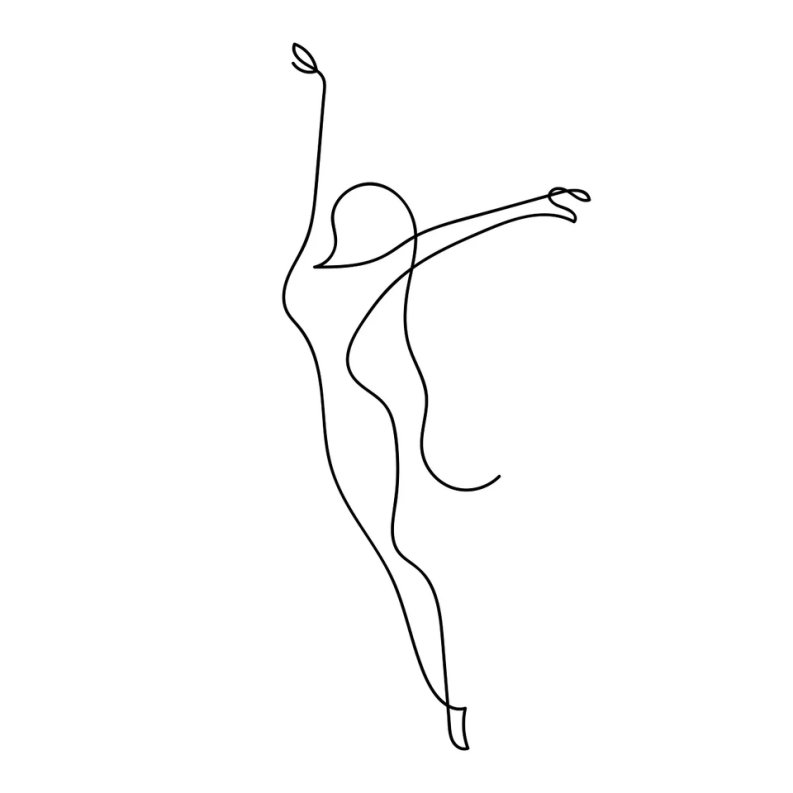
\includegraphics[width=0.2\textwidth]{Bailarina.png} 
    \caption{Imagen Bailarina utilizada en prueba 2}
    \label{fig:mi_imagen}
\end{figure}

 Y se utilizaron los siguientes datos para cada una de las 5 pruebas.

\begin{figure}[h]
    \centering
    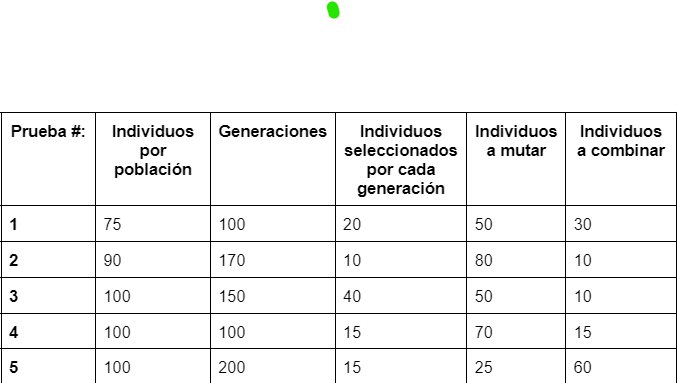
\includegraphics[width=0.480\textwidth, height=3cm]{tablaDatos.png} 
    \caption{Tabla con datos a utilizar en pruebas 1 y 2}
    \label{fig:mi_imagen}
\end{figure}

Luego de haber visto, se va a mostrar a continuación los resultados para cada computadora. Para ver los resultados de las pruebas realizadas donde se muestra la imagen de como quedó el dibujo se puede ver en la sección de anexos

\subsection{Computadora 1:}
Para la computadora 1 se hizo muestra el resultado para cada una de las pruebas. En la primera tabla se mostrará los resultados de la tabla de la imagen de la Hoja y para la segunda tabla se mostrará los resultados para la tabla de la bailarina. 

\begin{figure}[h]
    \centering
    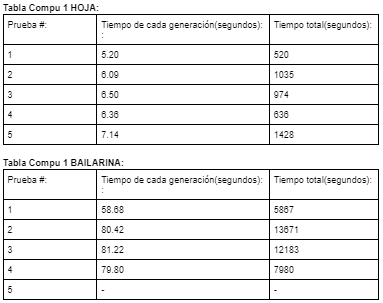
\includegraphics[width=0.480\textwidth, height=6cm]{tabla compu 1.png} 
    \caption{Resultados Compu 1}
    \label{fig:mi_imagen}
\end{figure}



\subsection{Computadora 2:}
Para la computadora 2 se hizo muestra el resultado para cada una de las pruebas. En la primera tabla se mostrará los resultados de la tabla de la imagen de la Hoja y para la segunda tabla se mostrará los resultados para la tabla de la bailarina. 


\begin{figure}[h]
    \centering
    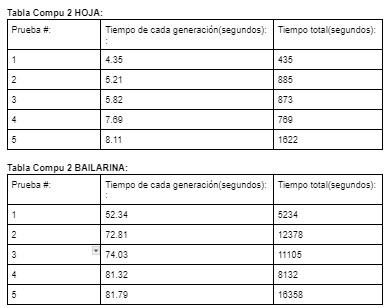
\includegraphics[width=0.480\textwidth, height=6cm]{tabla compu 2.png} 
    \caption{Resultados Compu 2}
    \label{fig:mi_imagen}
\end{figure}





 \subsection{Computadora 3:}
En la primera tabla se mostrará los resultados de la tabla de la imagen de la Hoja y para la segunda tabla se mostrará los resultados para la tabla de la bailarina. 


\begin{figure}[h]
    \centering
    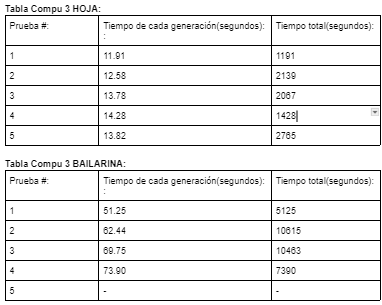
\includegraphics[width=0.480\textwidth, height=6cm]{tabla compu 3.png} 
    \caption{Resultados Compu 3}
    \label{fig:mi_imagen}
\end{figure}

\section{Analisis de resultados}\label{SCM}
Debido a la densidad de pixeles de las imágenes usadas, las pruebas a la imagen de "la hoja" tuvieron tiempos de finalización mucho menores a las de la imagen de "la bailarina", esto debido a que el fitness funciona comparando píxel por píxel las dimensiones de las imágenes a usar, por lo que estas terminan siendo un factor importante en el rendimiento del programa, también, un aspecto a tomar en cuenta para medir el tiempo de ejecución es cuantos individuos tiene cada generación ya que entre más aumenten, más tiempo le toma al programa generar cada nueva generación, a su vez, hay que considerar la cantidad de generaciones a realizar, ya que el tiempo de ejecución aumenta según cuantas generaciones se realicen, por lo que ambos aspectos van de la mano a la hora de aumentar o disminuir el tiempo de ejecución de pruebas en el programa .
Como se ve en las Fig. 4. y Fig. 5. Las pruebas realizadas fueron cinco en total y se hicieron en 3 computadoras con diferentes componentes para medir el rendimiento del programa en distintas computadoras y retornó los resultados mostrados, variando mucho entre las computadoras 1 y 2 con la computadora 3, ya que esta es la que cuenta con una mayor diferencia entre sus componentes, los resultados de las computadoras 1 y 2 son muy similares ya que la diferencia entre estas es solamente la cantidad de memoria RAM insertada en cada una.
Lo dicho anteriormente sobre el aumento en el tiempo de ejecución según los parámetros insertados en la cantidad de generaciones y los individuos de las mismas, se denota en las tablas, ya que muestra de forma gráfica las variaciones en el tiempo según los datos de entrada de cada prueba.
Cabe resaltar que la prueba 5 realizada a la bailarina tuvo el menor tiempo de ejecución en la computadora 3 ya que esta no fue capaz de terminarla satisfactoriamente y también en la máquina 1 debido a que por falta de tiempo no se pudo terminar de realizar la prueba, sin embargo, es de esperar que esta obtenga un resultado muy similar al obtenido por la computadora 2 por el tema de componentes explicado anteriormente.
Por último, también cabe destacar los resultados obtenidos cuando el algoritmo sacó las imagenes, como se observa en los anexos, las imagenes tuvieron algún parecido, pero no muy grande con la imagen original. Creemos que era imposible conseguir replicarla ya que las imagenes tenian una complejidad muy grande para poder conseguirlo en menos de 200 intentos y ocuparía una cantidad enorme de pruebas para lograrse, sin embargo cuando había más generaciones, se podía observar como se tenía una imagen más parecida a la original en comparación a cuando habia menos generaciones. Por eso la imagen que salió de la prueba 4 tiene más parecido a la imagen verdadera que la prueba 1 por ejemplo. 
\begin{figure}[h]
    \centering
    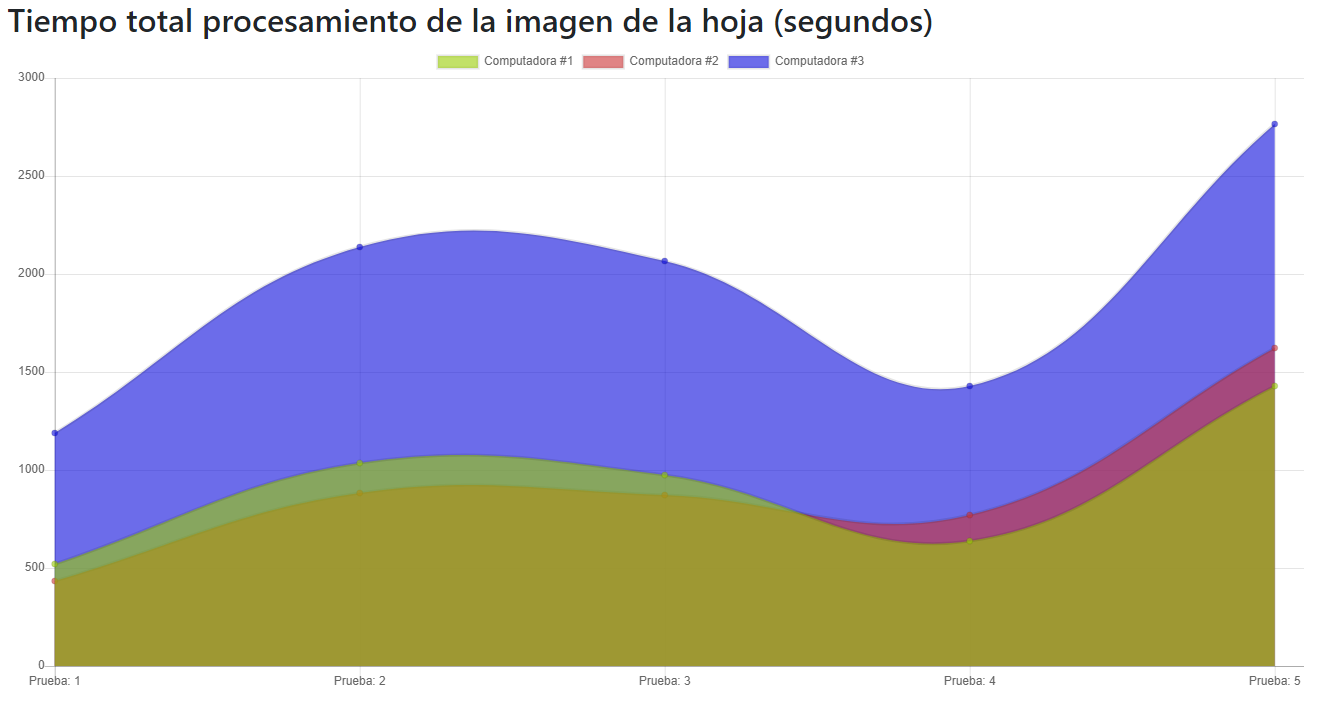
\includegraphics[width=0.480\textwidth, height=3cm]{tablaHoja.png} 
    \caption{Tiempo en segundos de las pruebas realizadas en cada computadora}
    \label{fig:mi_imagen}
\end{figure}

\begin{figure}[h]
    \centering
    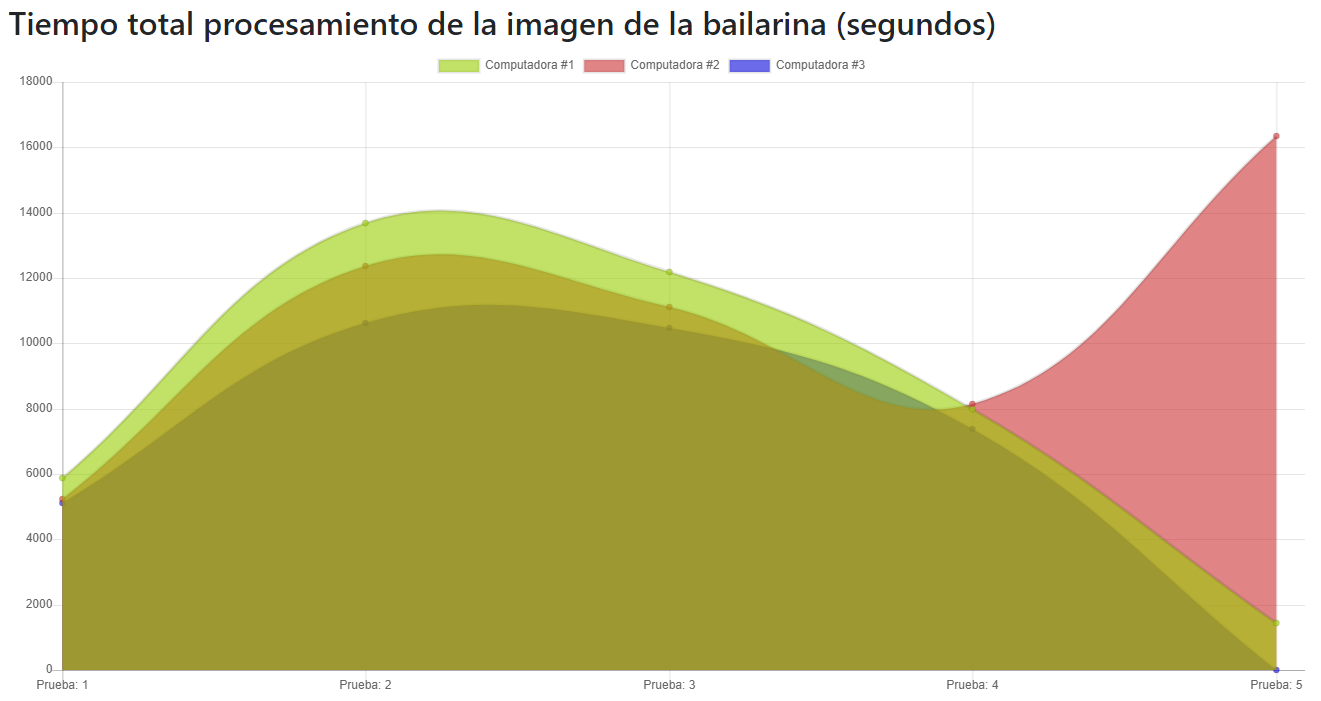
\includegraphics[width=0.480\textwidth, height=3cm]{tablaBailarina.png} 
    \caption{Tiempo en segundos de las pruebas realizadas en cada computadora}
    \label{fig:mi_imagen}
\end{figure}

\section{Conclusiones}
En conclusión, la implementación del algoritmo genético ha otorgado aprendizaje nuevo para los involucrados. Se ha experimentado y comprendido la funcionalidad de la aleatoriedad en este tipo de algoritmos, esto mediante las distintas pruebas realizadas con imágenes. 

La realización de estas pruebas ayudó tambien a visualizar de forma más detallada lo relacionado a tiempos de ejecución y se pudo lograr visualizar de forma directa como este es capaz de cambiar segun el tamaño de las diferentes instancias del problema, se logró ver como afectó cada una al tiempo final de ejecución lo que hace que funcione como un ejemplo directo del contexto.

Se pudo observar el efecto que tiene el dejar al algoritmo evolucionar y crear generaciones al momento de tratar de replicar la imagen enviada, se puede ver en las imagenes de los anexos como es que se logran resultados mejores con una mayor cantidad de generaciones comparados a los resultados con pocas generaciones, lo que genera la certeza de que con una cantidad mayor, mas no se sabe exactamente cuanto, de generaciones, el programa sería totalmente capaz de replicar la imagen en algun punto de forma muy fiel.

Además se pudo observar la importancia que tiene un buen hardware a la hora de realizar estas pruebas de algoritmos genéticos, ya que como se pudo observar se sugiere que los componentes del sistema, como la capacidad de la CPU y la cantidad de RAM, son factores cruciales. Esto destaca la necesidad de considerar cuidadosamente la infraestructura de hardware al seleccionar o diseñar algoritmos genéticos para aplicaciones específicas y no solo de algoritmos genéticos, si no que para tener el mejor rendimiento y optimización de un algoritmo va de la mano de un buen hardware. 

\section {Referencias}




\bibitem{b1} [1]S. Katoch, S. S. Chauhan, y V. Kumar, "A review on genetic algorithm: past, present, and future," Springer Science+Business Media, Oct. 2020.
\bibitem{b2}[2]V. M. Abascal Pelayo y P. Feijoo Ugalde, "Implementación de Algoritmos Genéticos sobre la plataforma de desarrollo paralelo CUDA," 2009.

\vspace{12pt}


\section {Anexos}


Luego aquí se muestra algunos ejemplos de como quedaron los dibujos realizados por los individuos y generaciones. Se mostrará la prueba 1 y 4 de cada una de las imagenes. 

\begin{figure}[h]
    \centering
    
\includegraphics[width=0.480\textwidth, height=6cm]{COMPU 1 HOJA-1.png} 
    \caption{Imagen Resultado Hoja Compu 1 Prueba 1}
    \label{fig:mi_imagen}
\end{figure}

\begin{figure}[h]
    \centering
    
\includegraphics[width=0.480\textwidth, height=6cm]{1 hoja compu1 .png} 
    \caption{Imagen Resultado Hoja Compu 1 Prueba 4}
    \label{fig:mi_imagen}
\end{figure}

\begin{figure}[h]
    \centering
    
\includegraphics[width=0.480\textwidth, height=6cm]{prueba 1 compu 1 bailarina.png} 
    \caption{Imagen Resultado Bailarina Compu 1 Prueba 1}
    \label{fig:mi_imagen}
\end{figure}

\begin{figure}[h]
    \centering
    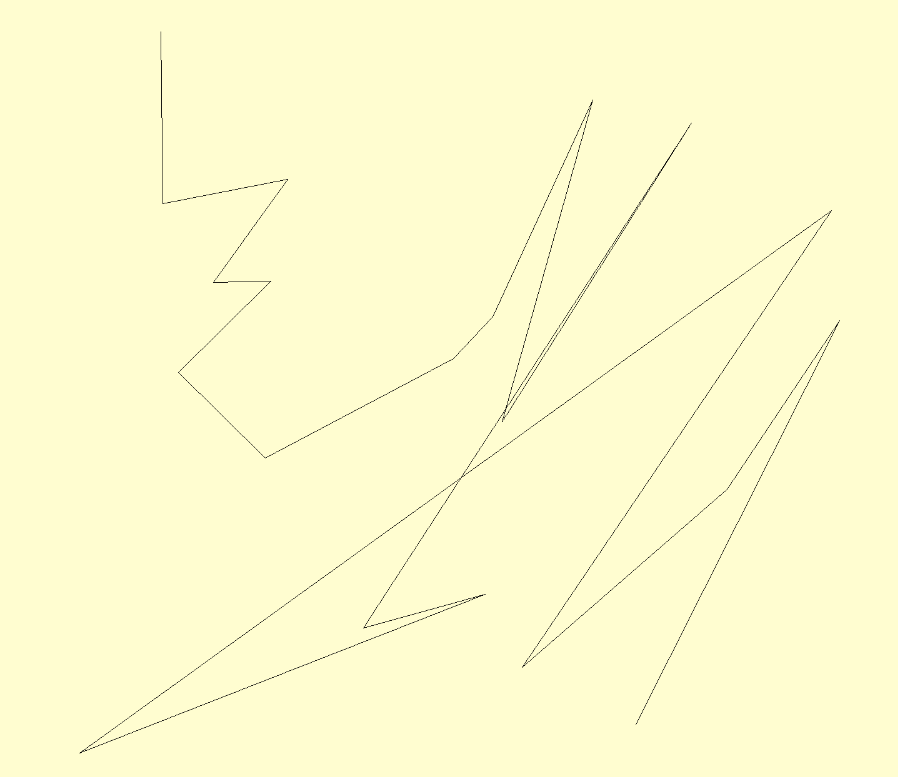
\includegraphics[width=0.480\textwidth, height=6cm]{bailarina compu 1 prueba 4.png} 
    \caption{Imagen Resultado Bailarina Compu 1 Prueba 4}
    \label{fig:mi_imagen}
\end{figure}


\begin{figure}[h]
    \centering
    
\includegraphics[width=0.480\textwidth, height=6cm]{unoCompu2Hoja.png} 
    \caption{Imagen Resultado Hoja Compu 2 Prueba 1}
    \label{fig:mi_imagen}
\end{figure}

\begin{figure}[h]
    \centering
    
\includegraphics[width=0.480\textwidth, height=6cm]{CuatroHojaCompu2.png} 
    \caption{Imagen Resultado Hoja Compu 2 Prueba 4}
    \label{fig:mi_imagen}
\end{figure}

\begin{figure}[h]
    \centering
    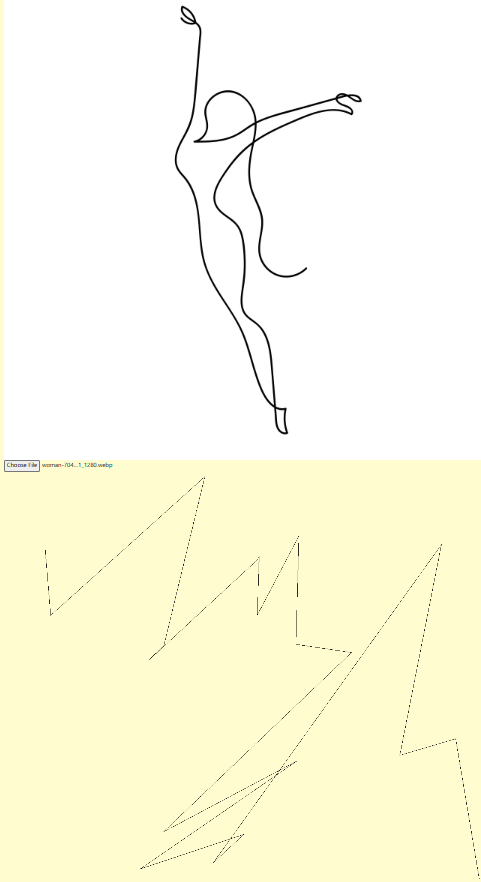
\includegraphics[width=0.480\textwidth, height=6cm]{unoBailarinaCompu2.png} 
    \caption{Imagen Resultado Bailarina Compu 2 Prueba 1}
    \label{fig:mi_imagen}
\end{figure}

\begin{figure}[h]
    \centering
    
\includegraphics[width=0.480\textwidth, height=6cm]{cuatroBailCompu2.png} 
    \caption{Imagen Resultado Bailarina Compu 2 Prueba 4}
    \label{fig:mi_imagen}
\end{figure}

\begin{figure}[h]
    \centering
    
\includegraphics[width=0.480\textwidth, height=6cm]{hoja-1-compu3.png} 
    \caption{Imagen Resultado Hoja Compu 3 Prueba 1}
    \label{fig:mi_ima{Imagen Resultado Hoja Compu 1 Prueba 1}gen}
\end{figure}

\begin{figure}[h]
    \centering
    
\includegraphics[width=0.480\textwidth, height=6cm]{hoja-4-compu3.png} 
    \caption{Imagen Resultado Hoja Compu 3 Prueba 4}
    \label{fig:mi_imagen}
\end{figure}

\begin{figure}[h]
    \centering
    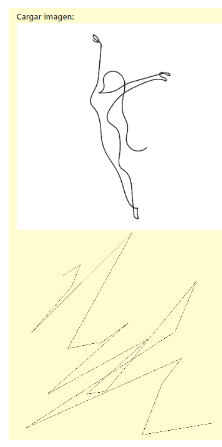
\includegraphics[width=0.480\textwidth, height=6cm]{bailarina-1-compu3.png} 
    \caption{Imagen Resultado Bailarina Compu 3 Prueba 1}
    \label{fig:mi_imagen}
\end{figure}

\begin{figure}[h]
    \centering
    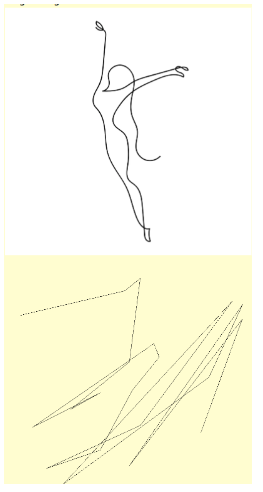
\includegraphics[width=0.480\textwidth, height=6cm]{bailarina-4-compu3.png} 
    \caption{Imagen Resultado Bailarina Compu 3 Prueba 4}
    \label{fig:mi_imagen}
\end{figure}




\end{document}
